\documentclass{article}

\usepackage{graphicx}
\usepackage{tikz}
\usepackage{tikzsymbols}
\usetikzlibrary{calc,patterns,shapes.geometric}
\pagestyle{empty}
\usepackage[margin=0pt]{geometry}
\geometry{papersize={14in,12in}}

\def\centerarc[#1](#2)(#3:#4:#5){\draw[#1] ($(#2)+({#5*cos(#3)},{#5*sin(#3)})$) arc (#3:#4:#5);}

\begin{document}
	\begin{figure}
		\centering
		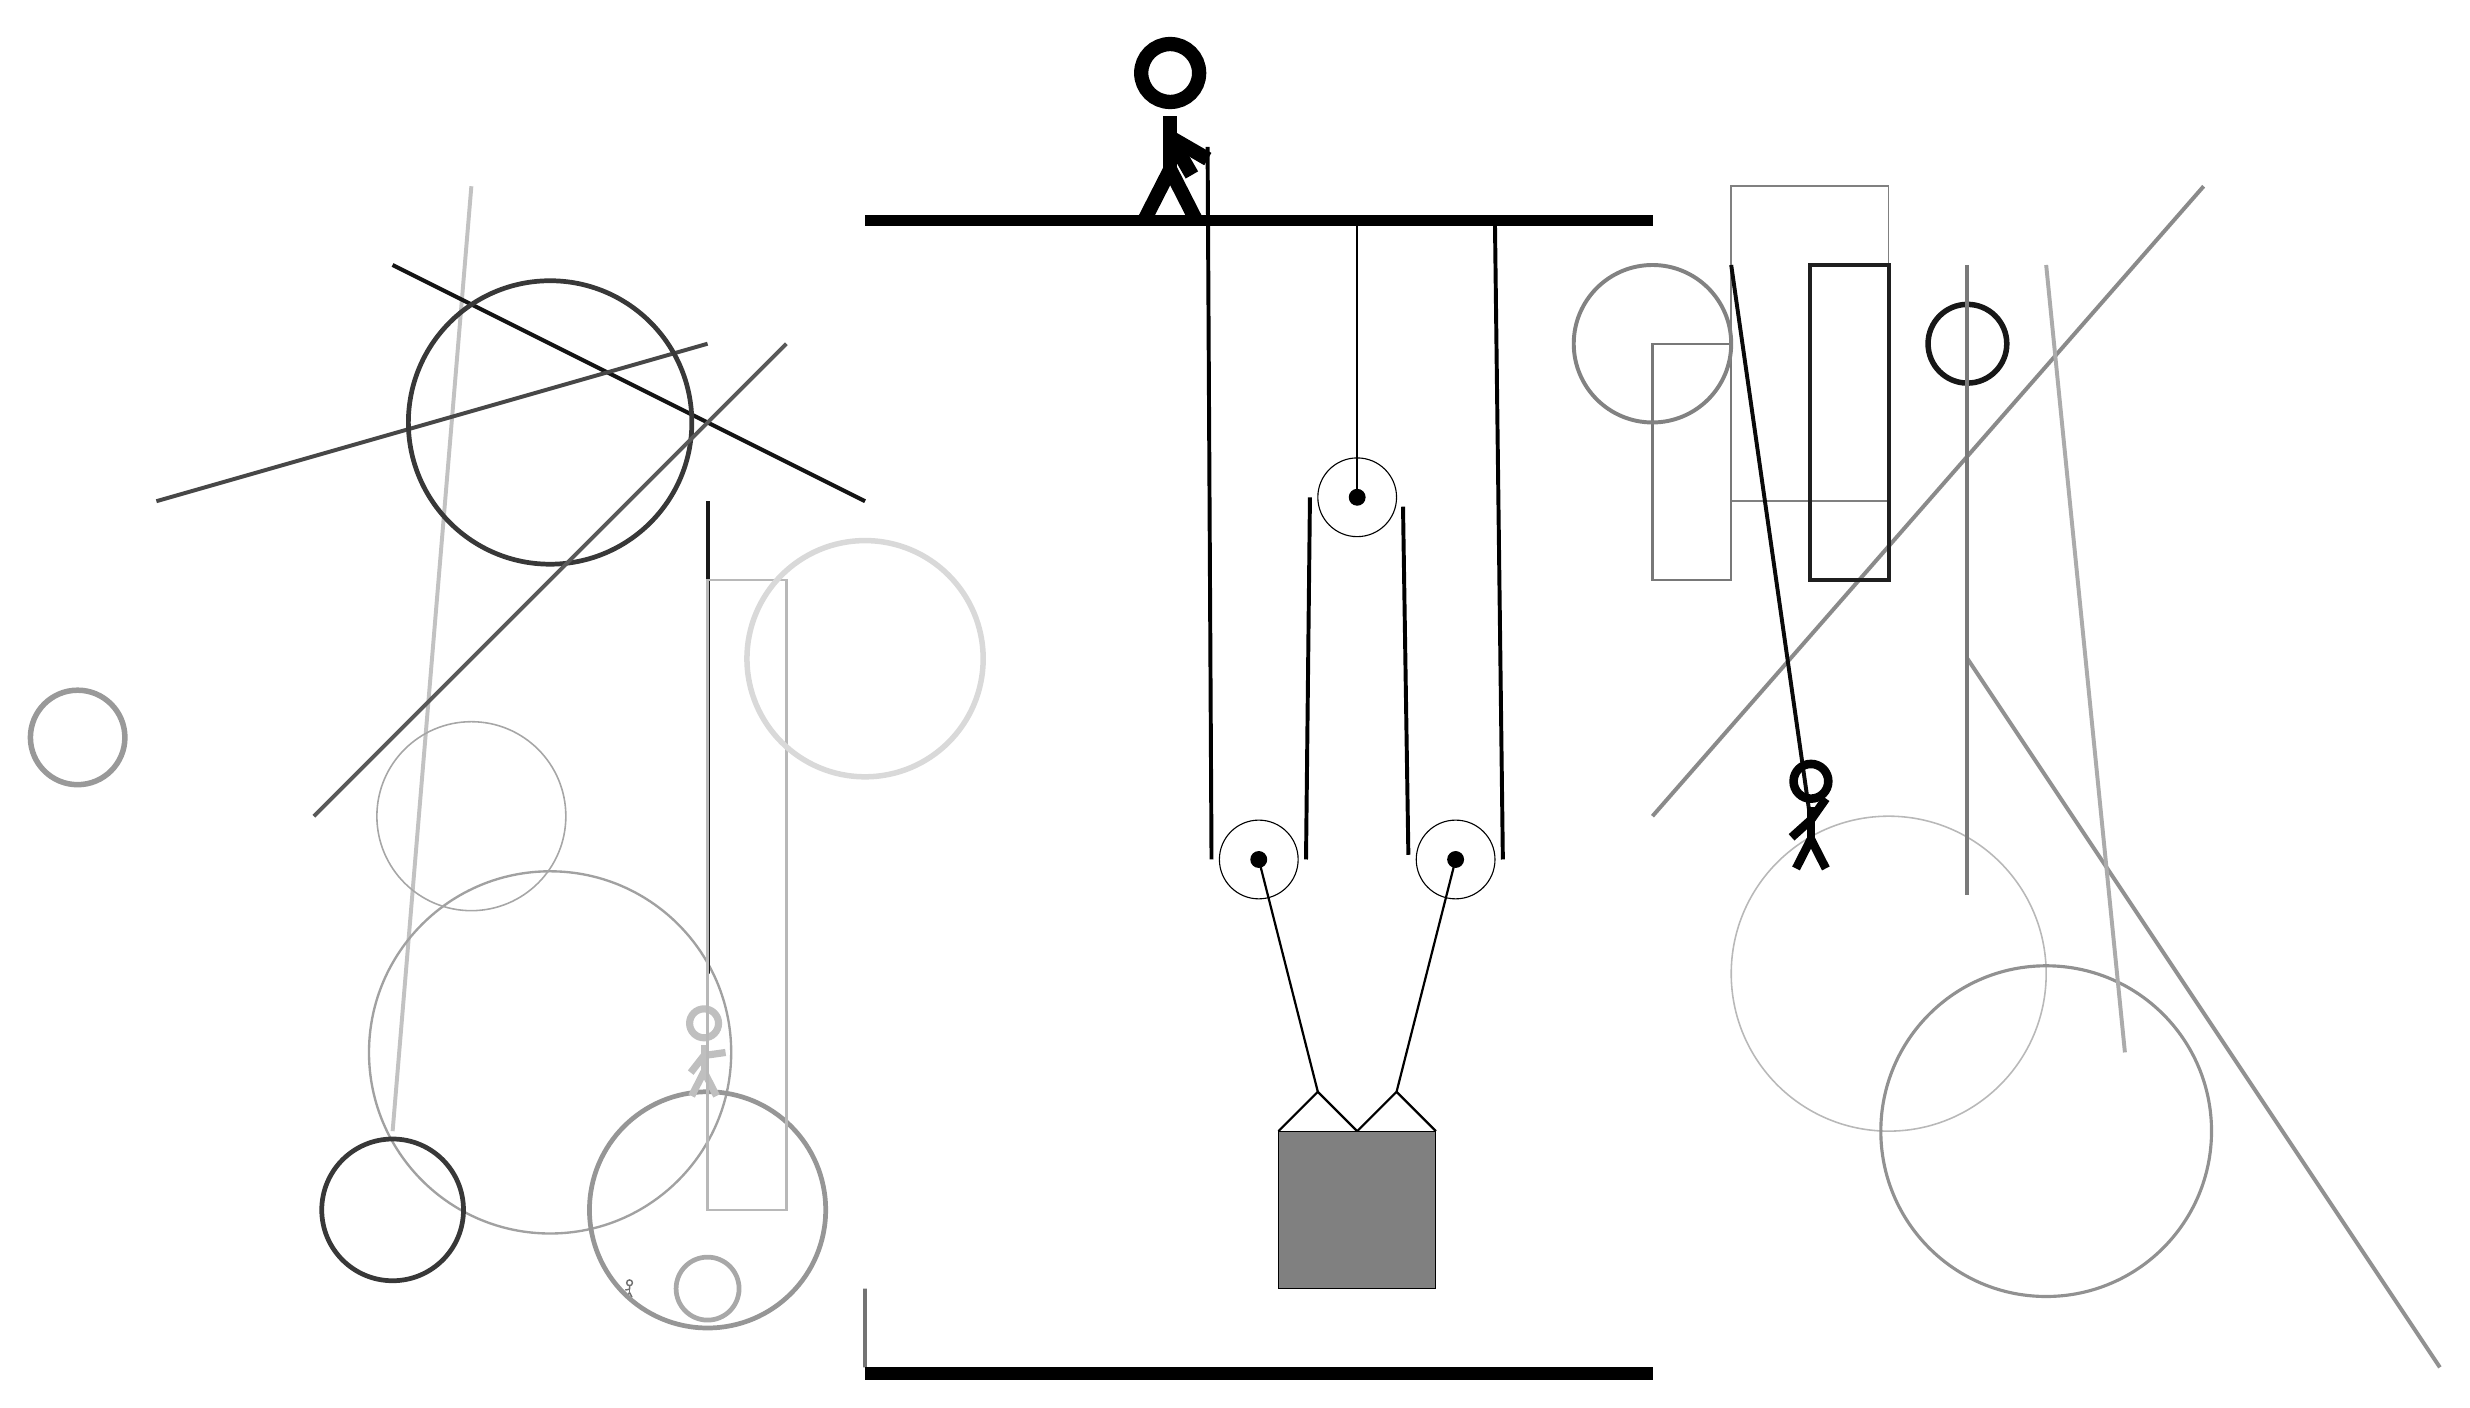
\begin{tikzpicture}
			%%%%% START %%%%%
			
			\draw[fill=black] (-4, 11.5) rectangle (6, 11.625);
			
			\draw (1, 3.45) circle (0.5);
			\draw[fill=black] (1, 3.45) circle (0.1);
			
			\draw (2.25, 8.05) circle (0.5);
			\draw[fill=black] (2.25, 8.05) circle (0.1);
			\draw[thick] (2.25, 8.05) -- (2.25, 11.5);
			
			\draw (3.5, 3.45) circle (0.5);
			\draw[fill=black] (3.5, 3.45) circle (0.1);
			
			\draw[line width=0.5mm, color=black!24](-9, 12) -- (-10, 0);
			
			\draw [line width=0.2mm, color=black!28](9, 2) circle (2.0);
			\draw[line width=0.5mm, color=black!46](6, 4) -- (13, 12);
			\draw [line width=0.7mm, color=black!91](10, 10) circle (0.5);
			\draw[line width=0.5mm, color=black!92](-4, 8) -- (-10, 11);
			\draw[line width=0.5mm, color=black!72](-6, 10) -- (-13, 8);
			
			\draw [line width=0.3mm, color=black!37](-8, 1) circle (2.3);
			\draw[line width=0.2mm, color=black!50] (7, 12) rectangle (9, 8);
			\draw[line width=0.5mm, color=black!96](7, 11) -- (8, 4);
			
			\node[line width=0.3mm, color=black!99] at (8, 4) {\Strichmaxerl[6][42][55]};
			\draw[line width=0.3mm, color=black!53] (7, 10) rectangle (6, 7);
			\node[line width=0.7mm, color=black!56] at (-7, -2) {\Strichmaxerl[1][10][86]};
			\draw [line width=0.6mm, color=black!78](-10, -1) circle (0.9);
			
			\draw [line width=0.4mm, color=black!43](11, 0) circle (2.1);
			\draw [line width=0.6mm, color=black!78](-8, 9) circle (1.8);
			\draw [line width=0.6mm, color=black!41](-6, -1) circle (1.5);
			\draw [line width=0.6mm, color=black!34](-6, -2) circle (0.4);
			\draw[line width=0.5mm, color=black!88] (8, 11) rectangle (9, 7);
			\draw[line width=0.5mm, color=black!43](10, 6) -- (16, -3);
			
			\draw[line width=0.5mm, color=black!33](11, 11) -- (12, 1);
			\draw[line width=0.5mm, color=black!55] (-4, -2) rectangle (-4, -3);
			
			\draw [line width=0.7mm, color=black!40](-14, 5) circle (0.6);
			\draw[line width=0.5mm, color=black!65](-5, 10) -- (-11, 4);
			\draw[line width=0.5mm, color=black!52](10, 11) -- (10, 3);
			\draw [line width=0.5mm, color=black!49](6, 10) circle (1.0);
			
			\draw[line width=0.5mm, color=black!90] (-6, 8) rectangle (-6, 2);
			\node[line width=0.6mm, color=black!25] at (-6, 1) {\Strichmaxerl[5][52][8]};
			\draw [line width=0.2mm, color=black!35](-9, 4) circle (1.2);
			\draw[line width=0.3mm, color=black!28] (-6, 7) rectangle (-5, -1);
			\draw [line width=0.7mm, color=black!15](-4, 6) circle (1.5);
			
			\draw[thick] (3.5, 3.45) -- (2.75, 0.5);
			\draw[thick] (1, 3.45) -- (1.75, 0.5);
			\draw[thick]  (1.25, 0) -- (1.75, 0.5) -- (2.25, 0);
			\draw[thick]  (2.25, 0) -- (2.75, 0.5) -- (3.25, 0);
			\draw[fill=black!50] (1.25, 0) rectangle (3.25, -2);
			
			\draw[line width=0.5mm] (0.35, 12.5) --  (0.4, 3.45);
			\centerarc[line width=0.5mm](1, 3.45)(180:360:0.6);
			\draw[line width=0.5mm] (1.6, 3.45) -- (1.65, 8.05);
			\centerarc[line width=0.5mm](2.25, 8.05)(-20:180:0.6);
			\draw[line width=0.5mm](2.832, 7.93) -- (2.9, 3.51);
			\centerarc[line width=0.5mm](3.5, 3.45)(160:360:0.6);
			\draw[line width=0.5mm](4.1, 3.45) -- (4.0, 11.5);
			
			\node at (-0.07, 12.7) {\Strichmaxerl[10][120][-30]};
			
			\draw[fill=black] (-4, -3) rectangle (6, -3.15);
			
			%%%%% END %%%%%
		\end{tikzpicture}
	\end{figure}	
\end{document}